% This file was created with matplot2tikz v0.4.0.
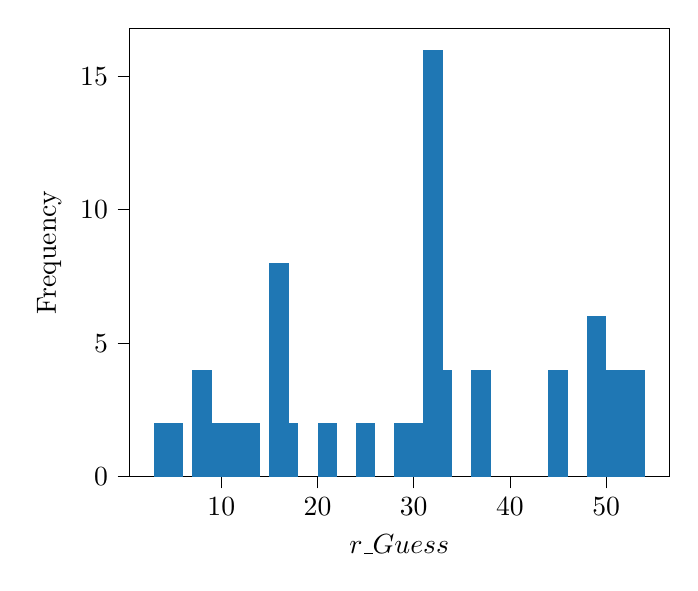
\begin{tikzpicture}

\definecolor{darkgray176}{RGB}{176,176,176}
\definecolor{steelblue31119180}{RGB}{31,119,180}

\begin{axis}[
tick align=outside,
tick pos=left,
x grid style={darkgray176},
xlabel={\(\displaystyle r\_{Guess}\)},
xmin=0.45, xmax=56.55,
xtick style={color=black},
y grid style={darkgray176},
ylabel={Frequency},
ymin=0, ymax=16.8,
ytick style={color=black}
]
\draw[draw=none,fill=steelblue31119180] (axis cs:3,0) rectangle (axis cs:5,2);
\draw[draw=none,fill=steelblue31119180] (axis cs:4,0) rectangle (axis cs:6,2);
\draw[draw=none,fill=steelblue31119180] (axis cs:7,0) rectangle (axis cs:9,4);
\draw[draw=none,fill=steelblue31119180] (axis cs:8,0) rectangle (axis cs:10,2);
\draw[draw=none,fill=steelblue31119180] (axis cs:10,0) rectangle (axis cs:12,2);
\draw[draw=none,fill=steelblue31119180] (axis cs:12,0) rectangle (axis cs:14,2);
\draw[draw=none,fill=steelblue31119180] (axis cs:15,0) rectangle (axis cs:17,8);
\draw[draw=none,fill=steelblue31119180] (axis cs:16,0) rectangle (axis cs:18,2);
\draw[draw=none,fill=steelblue31119180] (axis cs:20,0) rectangle (axis cs:22,2);
\draw[draw=none,fill=steelblue31119180] (axis cs:24,0) rectangle (axis cs:26,2);
\draw[draw=none,fill=steelblue31119180] (axis cs:28,0) rectangle (axis cs:30,2);
\draw[draw=none,fill=steelblue31119180] (axis cs:30,0) rectangle (axis cs:32,2);
\draw[draw=none,fill=steelblue31119180] (axis cs:31,0) rectangle (axis cs:33,16);
\draw[draw=none,fill=steelblue31119180] (axis cs:32,0) rectangle (axis cs:34,4);
\draw[draw=none,fill=steelblue31119180] (axis cs:36,0) rectangle (axis cs:38,4);
\draw[draw=none,fill=steelblue31119180] (axis cs:44,0) rectangle (axis cs:46,4);
\draw[draw=none,fill=steelblue31119180] (axis cs:48,0) rectangle (axis cs:50,6);
\draw[draw=none,fill=steelblue31119180] (axis cs:49,0) rectangle (axis cs:51,2);
\draw[draw=none,fill=steelblue31119180] (axis cs:50,0) rectangle (axis cs:52,4);
\draw[draw=none,fill=steelblue31119180] (axis cs:52,0) rectangle (axis cs:54,4);
\end{axis}

\end{tikzpicture}
